Os principais componentes das máquinas de corrente alternada assíncronas estão o rotor e o estator. O rotor, por definição, é a peça que gira em torno do seu próprio eixo. A máquina de indução, ao contrário da máquina CC, possui um entreferro uniforme. O rotor pode ser do tipo gaiola de esquilo ou do tipo bobinado.
    
Os enrolamentos do estator aa’, bb’ e cc’ estão defasados de 120 graus entre si. Quando uma corrente alternada passa por um enrolamento ela produz uma força magneto-motriz também alternada e centrada no eixo do enrolamento. Cada força magneto-motriz é representada por um vetor com magnitude proporcional ao valor instantâneo da corrente. As correntes instantâneas em cada enrolamento são mostradas na figura \ref{fig:11}.

\begin{figure}[hbt]
    \center 
    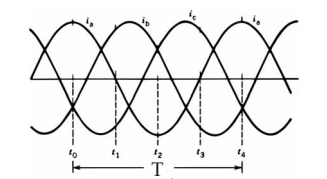
\includegraphics[scale=1.2]{imagens/11.PNG}
    \caption{Correntes instantâneas em cada enrolamento.}\label{fig:11}
\end{figure}

A força magneto-motriz resultante é composta pelas três componentes de força
magneto-motriz, que pode ser visualizada graficamente como na figura \ref{fig:12}.

\begin{figure}[ht]
    \center 
    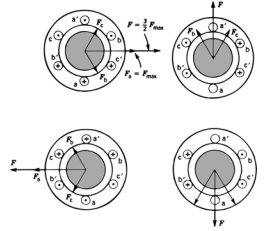
\includegraphics[scale=1.2]{imagens/12.PNG}
    \caption{Campo magnético girante.}\label{fig:12}
\end{figure}

No instante de tempo $t_o$, a corrente na fase a passa por um máximo positivo e as correntes nas fases b e c por metade da amplitude máxima negativa. Devido ao fato da corrente na fase a estar em um instante de máximo, a força magneto-motriz produzida por este enrolamento é máxima.

A força magneto-motriz, resultante da composição vetorial das forças magneto-motriz devido aos três enrolamentos, é dada pela equação
$$\vec{F} = \frac{2}{3}.F_{max}$$

A força magneto-motriz resultante é distribuída senoidalmente ao longo do entreferro. Analisando o que acontece à medida que as correntes em cada enrolamento variam senoidalmente, nota-se que o vetor resultante F possui a mesma amplitude em todos os
instantes de tempo, mas ele gira em sentido anti-horário.

